\begin{frame}{Monge's Orthoptic Circle \href{https://youtu.be/9fI3iM2jrmI}{[video]}}
\begin{tabular}{cl}
\begin{tabular}{c}
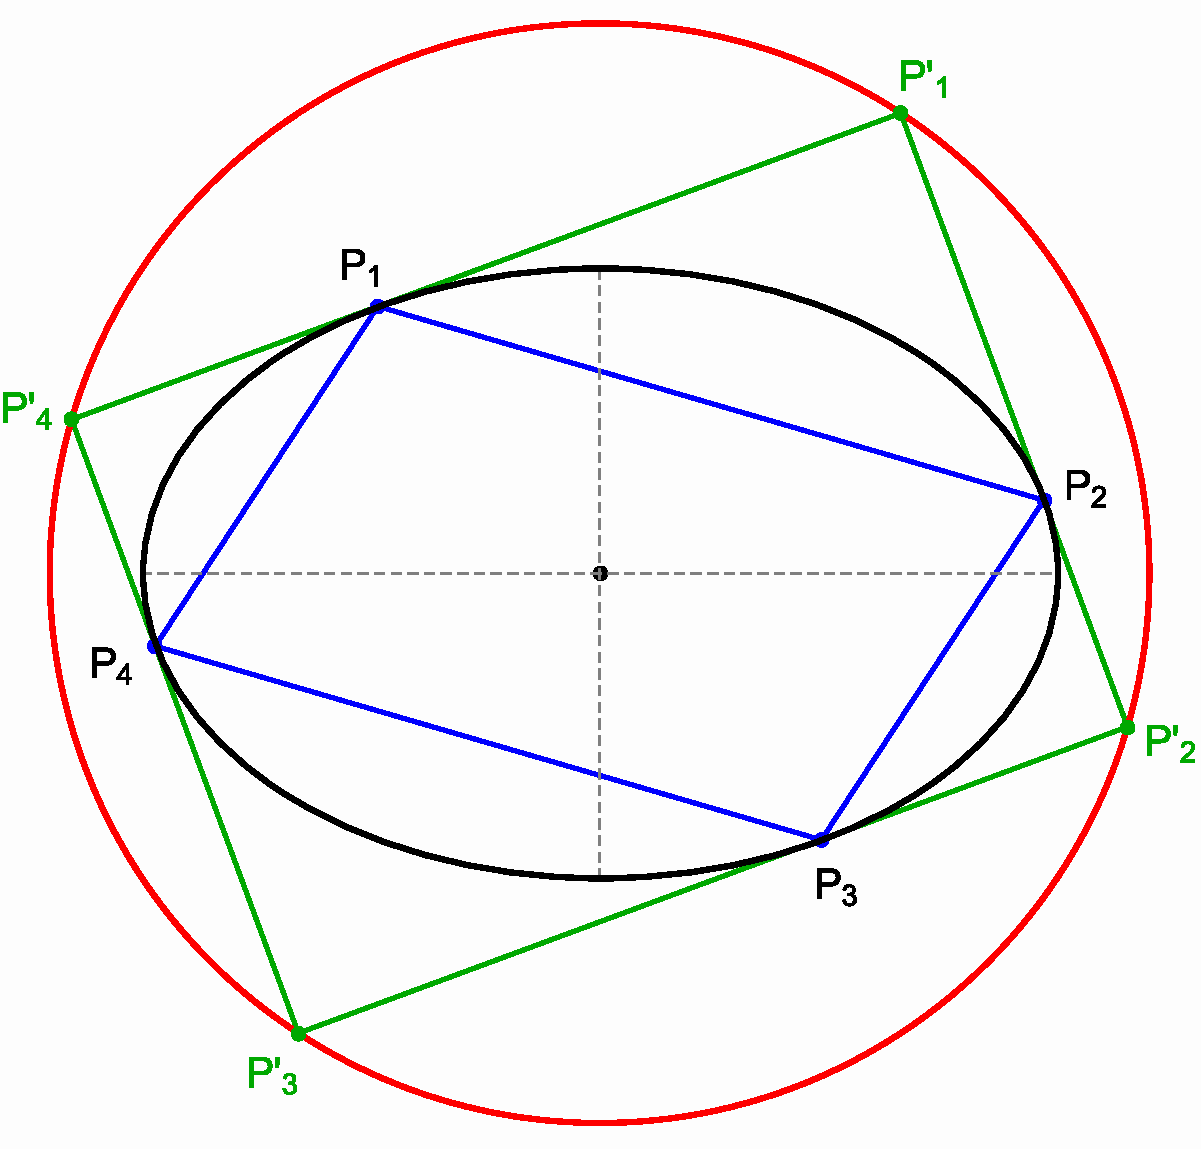
\includegraphics[height=.8\textheight]{pics/0200_monge_orthoptic.pdf}
\end{tabular} & \begin{tabular}{l}
\parbox{0.5\linewidth}{
  \begin{minipage}{0.5\textwidth}
 \begin{itemize}
    \item * Stationary Circle
    \item * Rectangle diagonals.
    \item * $\sum{\cos{\theta_i}}=0$.
    \item * $\prod{\cos{\theta_i'}}=0$.
\end{itemize}
\end{minipage}}
\end{tabular}  \\
\end{tabular}
\end{frame}

\begin{frame}{Generalized Stationary Circle     \href{https://youtu.be/dINE4aH1cvk}{[video 1]} and \href{https://youtu.be/EFeINGIDFrg}{[video 2]}}
\begin{figure}
    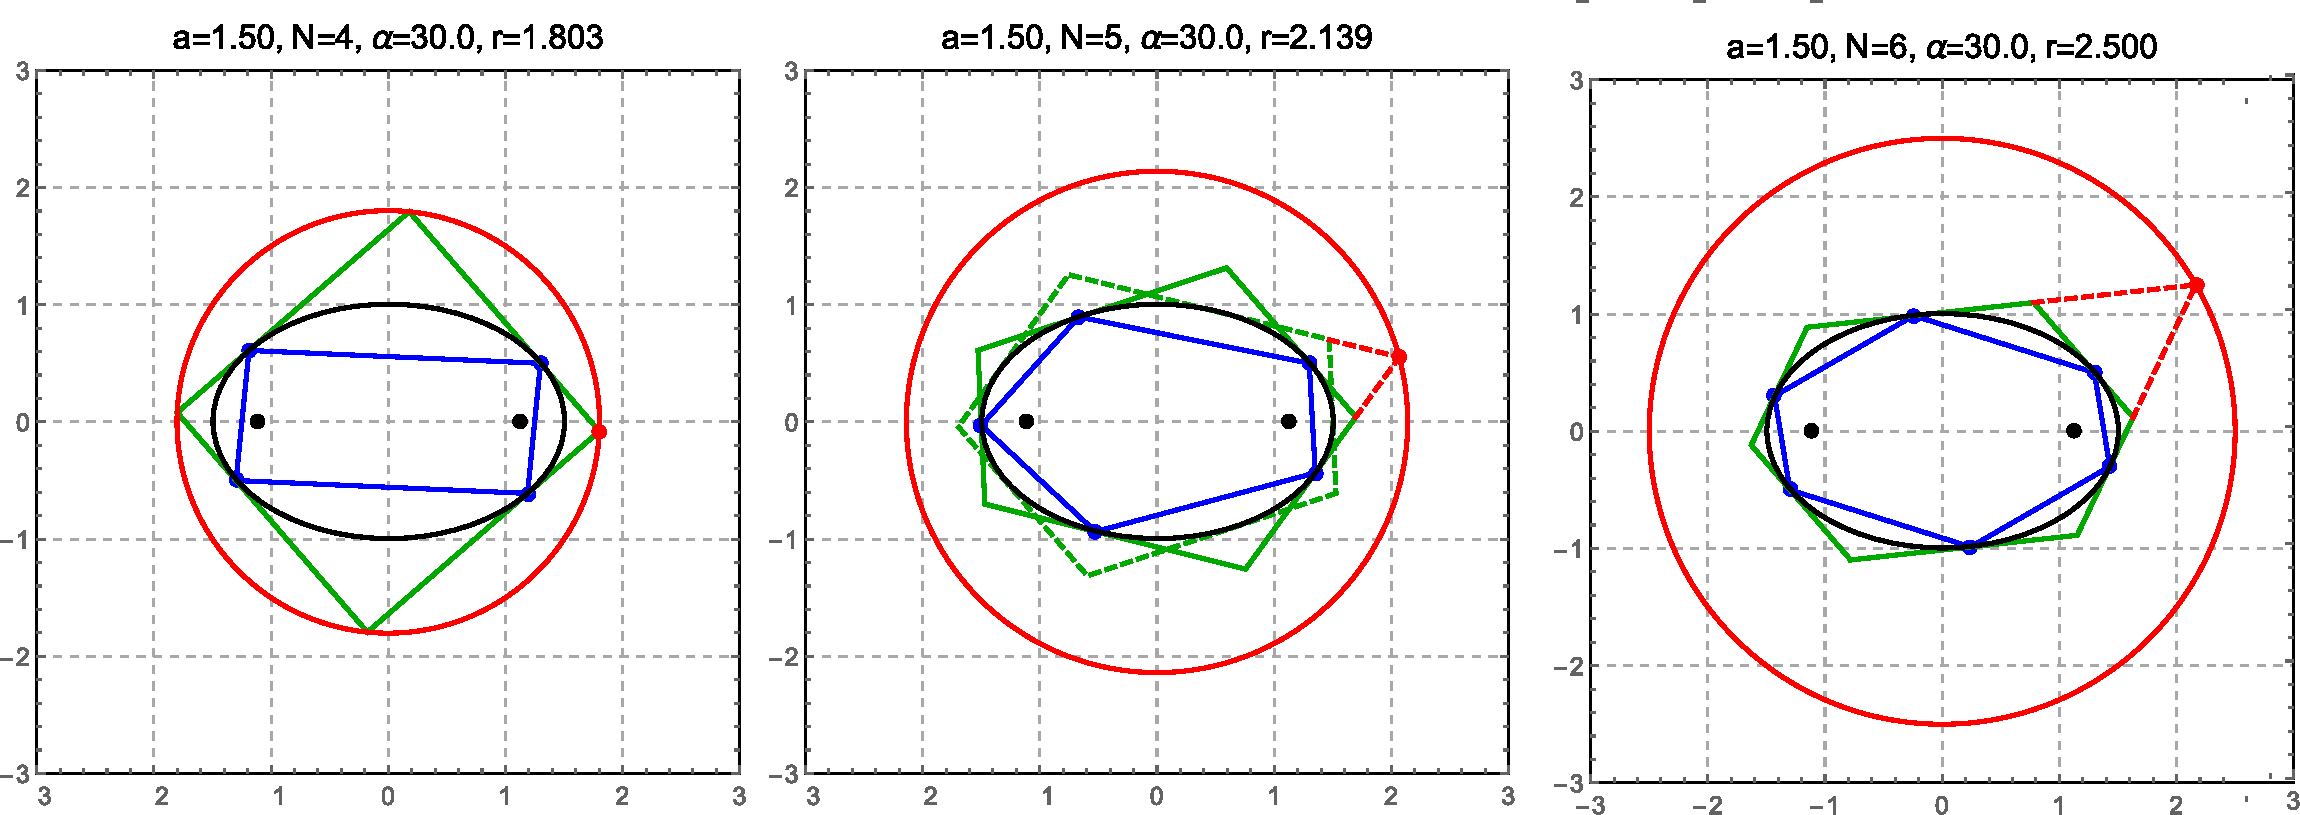
\includegraphics[clip,trim={0 0 0 1.66cm},width=\textwidth]{pics/0180_circ_grid_v3.pdf}
\end{figure}
\vspace*{-.125cm}
$\implies E\,'_{i}\cap-E\,'_{i+1}$ is a stationary circle of  $r^*=1/\gamma$
\end{frame}

\begin{frame}{$N>3$ Mittenpunkt \href{https://youtu.be/TV2p7fPlYfE}{[video 1]} and Extouchpoints \href{https://youtu.be/Bpc-MrR2IMc}{[video 2]}}
\begin{figure}
    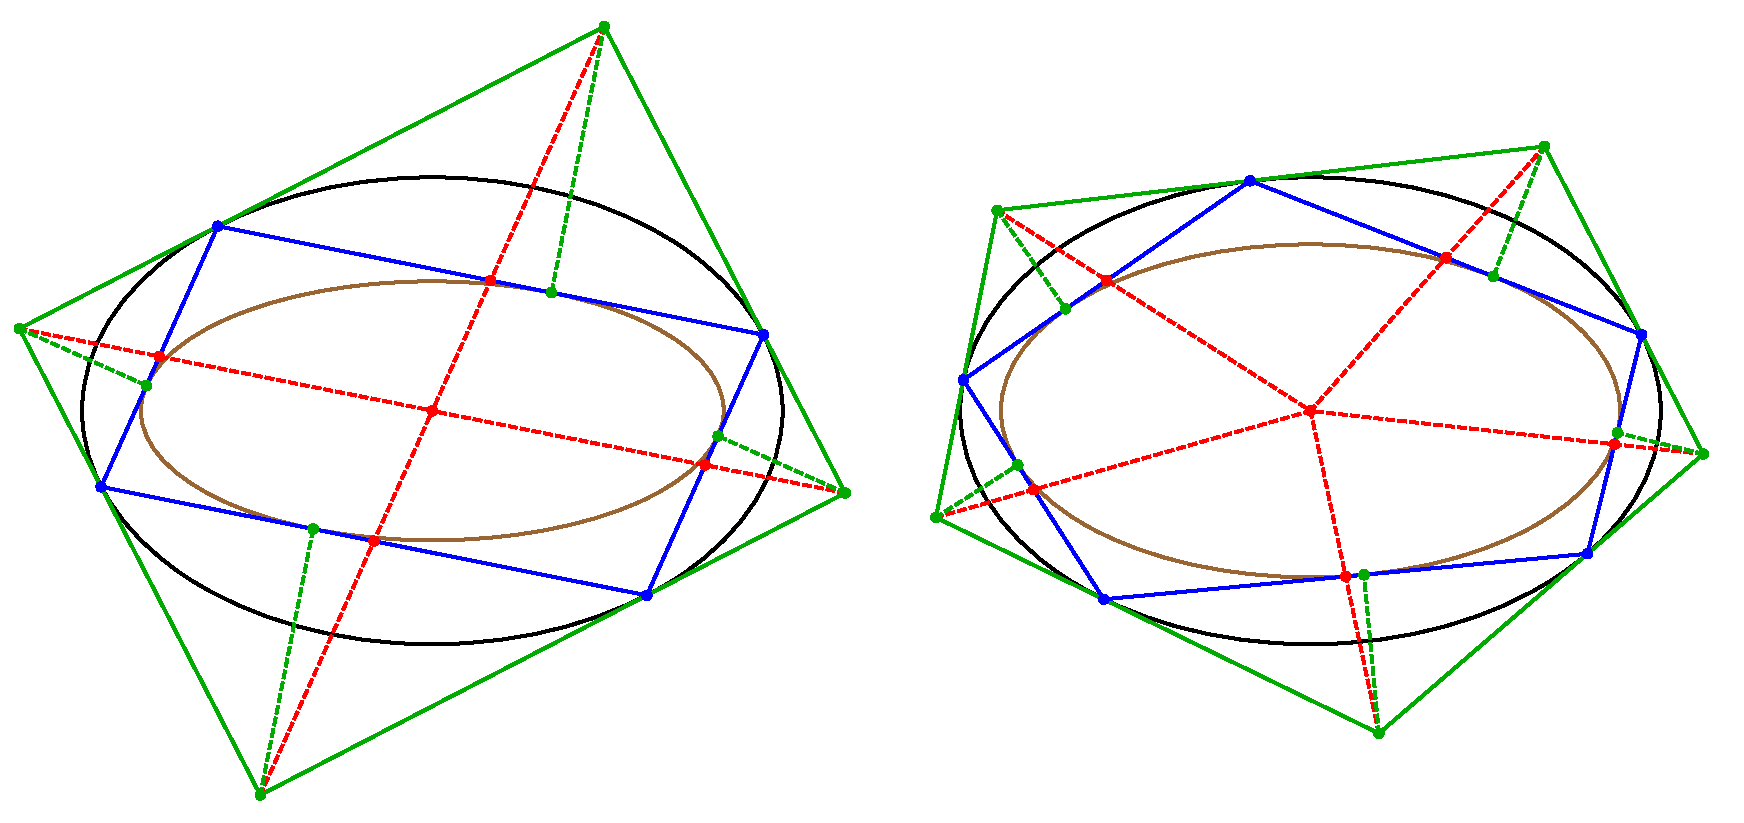
\includegraphics[width=\textwidth]{pics/0165_extouch.pdf}
    \label{fig:gen-mitten}
\end{figure}
\end{frame}

\begin{frame}{Cosine Sums for $N>3$}
\begin{figure}
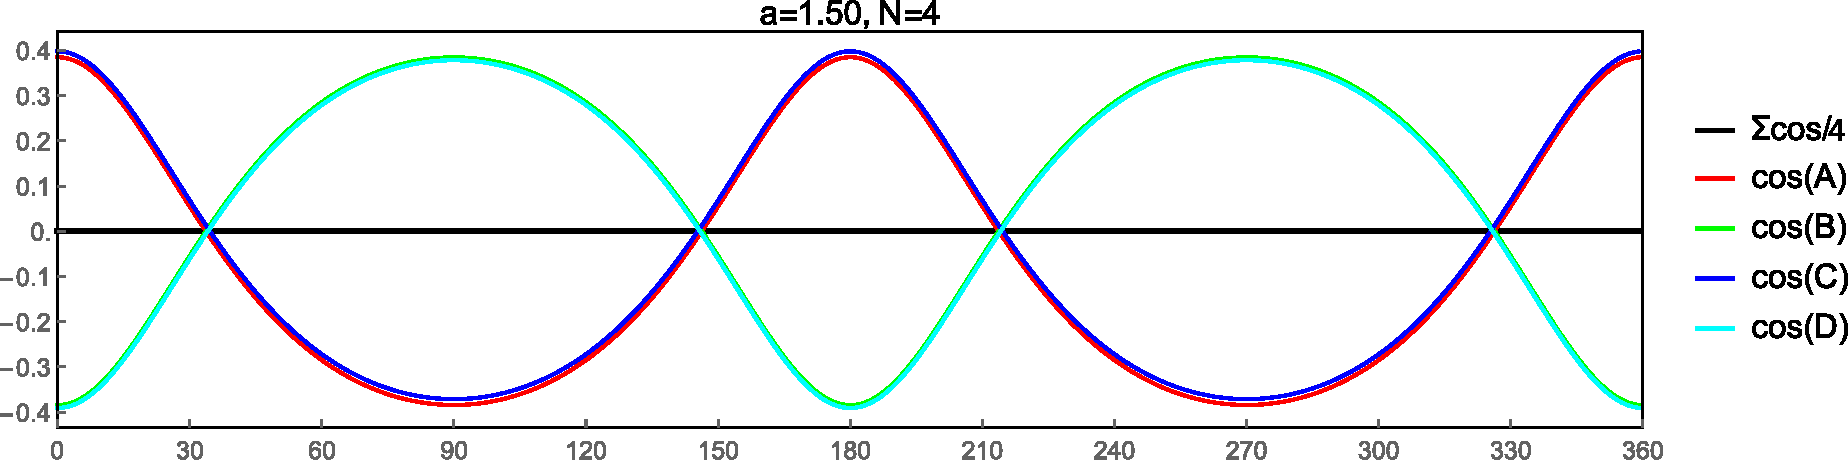
\includegraphics[width=.9\textwidth]{pics/0091_cosine_sum_n4.pdf}\\
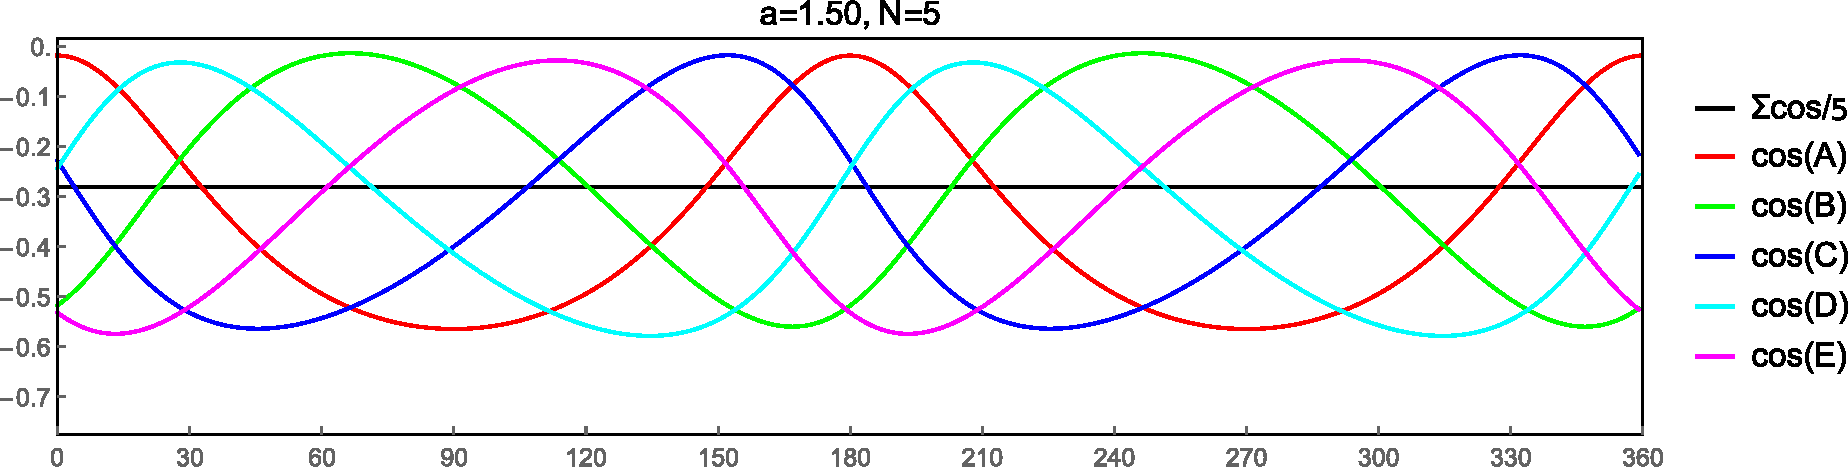
\includegraphics[width=.9\textwidth]{pics/0092_cosine_sum_n5.pdf}
\end{figure}
\end{frame}

\begin{frame}{Sum, Product, Area Ratios are Conserved!}
\begin{tabular}{cl}
\begin{tabular}{c}
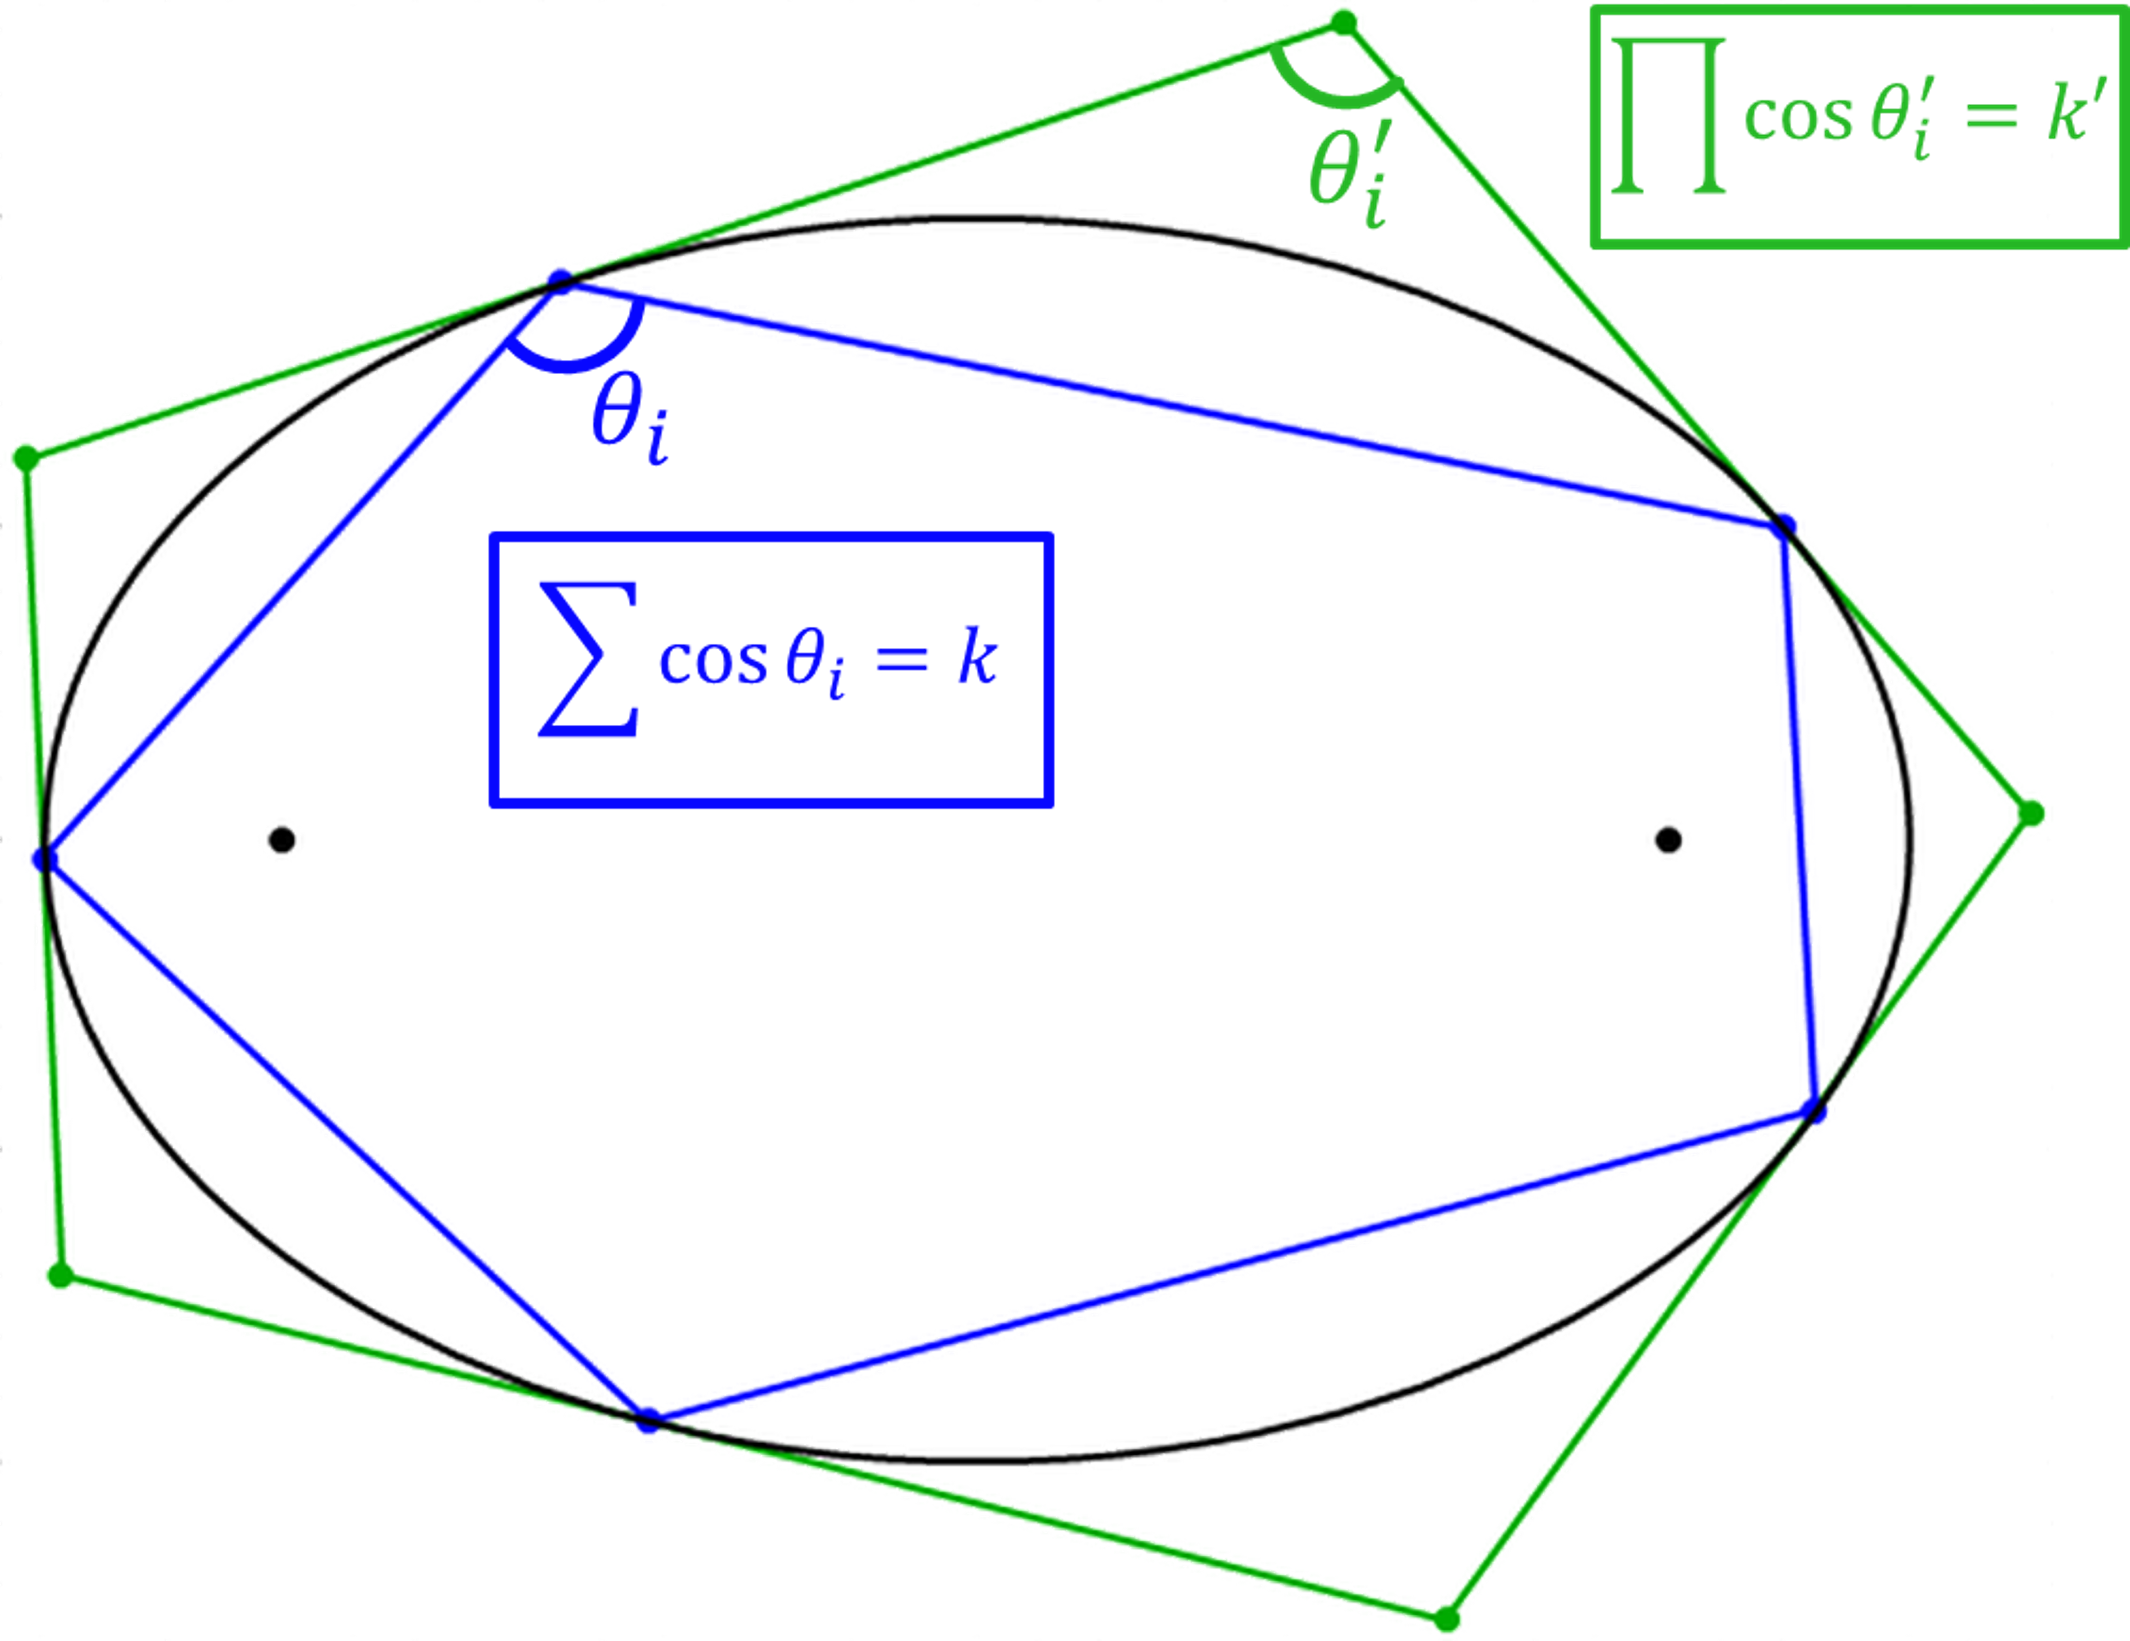
\includegraphics[height=.6\textheight]{pics/0078_cosine_sum_and_product_for_all_n.png}
\end{tabular} & \begin{tabular}{l}
\parbox{0.5\linewidth}{
  \begin{minipage}{0.5\textwidth}
\begin{itemize}
\item $\implies$ $\sum_{i=1}^{N}{\cos{\theta_i}}$ conserved  $\forall{N}$.
\item $\implies$ $\prod_{i=1}^{N}{\cos{\theta_i'}}$ conserved  $\forall{N}$.
\item $\implies$ $A'/A$ conserved $\forall{N}$ \textbf{odd}.
\end{itemize}
\end{minipage}}
\end{tabular}  \\
\end{tabular}
\end{frame}